\documentclass{article}
\usepackage{setspace}
\usepackage[text={6.5in,8.5in},centering]{geometry}
\geometry{verbose,a4paper,tmargin=2.4cm,bmargin=2.4cm,lmargin=2.4cm,rmargin=2.4cm}
\usepackage{graphicx,amsmath,cases,multirow,appendix,graphicx,xcolor}

\setlength\parindent{0pt}

\newcommand{\note}[1]{\colorbox{gray!30}{#1}}
\newcommand{\ind}{\-\hspace{1cm}}
\newcommand*{\blanks}[1][4em]{\rule{#1}{.4pt}}


\begin{document}

\noindent\makebox[\textwidth][c]{\Large\bfseries Quiz 2 - MSY Harvest Scenarios}

\rule[0.5ex]{\linewidth}{1pt}
\begin{center}
	\textbf{My name is:} \blanks[150pt]
\end{center}
\rule[0.5ex]{\linewidth}{1pt}

Assume that the curve (solid line) of the following figure reflects the underlying mean empirical relationship between the population growth rate ($dN/dt$) of a commercially-harvested fish species and its abundance ($N$).  Such a density-dependent relationship is often called the stock-recruitment function in fisheries management.  The labeled lines (\textbf{A} and \textbf{B}) illustrate two contrasting harvesting strategies that could be applied to this fishery.
\begin{center}
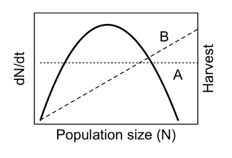
\includegraphics[width=6cm]{figs/image}\\
\end{center}
(a) Based on the slopes of the two lines, match these strategies to the following models describing the relationship between the population's recruitment rate ($dN/dt$) and its stock size ($N$), intrinsic growth rate ($r$), carrying capacity ($K$), and the rates of harvest ($h$ or $H$).
\begin{align*}
	\frac{dN}{dt}=rN \left(1-\frac{N}{K}\right)-hN &\quad \quad \quad &   \frac{dN}{dt}=rN \left(1-\frac{N}{K}\right)-H \\
	\text{Scenario: \textcolor{red}{B}} & \quad \quad \quad & \text{Scenario:\textcolor{red}{A} }
\end{align*}

\vspace{1cm}

(b) Describe these strategies \emph{in less than} 15 words each.\\
\ind Scenario A: \textcolor{red}{Fixed quota; Constant number of individuals harvested.} \\
\vspace{1cm}

\ind Scenario B: \textcolor{red}{Fixed effort quota; Constant proportion or fraction of population harvested.}\\
\vspace{1cm}

(c) Illustrate on the figure how the line for scenario \textbf{A} would change if harvesting pressure were to increase under this scenario.  Illustrate an increase for scenario \textbf{B}. \\
\textcolor{red}{For A, intercept increases and slope (=0) stays the same.}\\
\textcolor{red}{For B, slope increases and intercept (=0) stays the same.}\\

(d) Assuming that the stock-recruitment relationship depicted in the figure is indeed an adequate description of the empirical situation for this fishery, use your answer to the previous question to justify why one of the two scenarios (\textbf{A} or \textbf{B}) might be considered a more sustainable harvesting scenario than the other. 

\textcolor{red}{Both strategies are susceptible to overfishing if harvesting exceeds recruitment rates.
However, the total amount harvested per time-step by scenario \textbf{B} self-adjusts to the population size available; \textbf{B} removes a constant proportion of the population (assuming harvesting effort and catchability are indeed fixed).  Thus \textbf{B} is somewhat buffered against variation in the stock-recruitment relationship and/or short-term over-harvesting.}

\end{document}